\section{E-Logbook}
E-Logbook adalah sebuah buku elektronik untuk mencatat catatan/dokumen penting secara detail setiap aktivitas yang berisi masalah-masalah yang membutuhkan tindak lanjut dari pihak yang terlibat dalam satu hari penuh. Seluruh pegawai sebaiknya membaca buku ini agar mengetahui kegiatan, kerusakan, dan target pekerjaan apa saja yang dilakukan hari sebelumnya. Ada beberapa manfaat e-logbook antara lain:
\begin{enumerate}
\item bahan bukti untuk merekap seluruh aktivitas
\item bahan pembuatan laporan kegiatan
\item alat untuk memudahkan pegawai dalam merekap kegiatan
 \end{enumerate}

Hal yang perlu di isi dalam e-logbook ini antara lain:
\begin{enumerate}
\item Hari, tanggal dan tahun
\item Nama pegawai yang dinas pada hari tersebut
\item Nama vendor yang dinas pada hari tersebut
\item Penerbangan hari ini
\item Kegiatan
\item Kerusakan
\item Target pekerjaan
\end{enumerate}


\subsection{Mengaktifkan MySQLi}
Kenapa disini kita membahas tentang cara mengaktifkan MySQLi karena PHP 5 keatas default-nya menggunakan platform MySQLi untuk menggunakan berbagai fungsi pada database MySQL. MySQLi adalah sebuah class di PHP, jadi pastikan bahwa versi PHP kita sudah 5 keatas yaa.
Keunggulan menggunakan MySQLi ketimbang dengan MySQL:
\begin{enumerate}
\item Dukungan baru untuk keperluan transaksi
\item Prosedur interface
\item Susunan laporan lebih tersusun
\item Debugging lebih ditingkatkan
\item Dapat memproses dalam waktu yang lebih singkat
\end{enumerate}

Nah itu beberapa keunggulan menggunakan MySQLi. Dan sekarang kita akan membahas cara mengaktifkan MySQLi pada PHP.
Untuk mengaktifkan MySQLi, langkah pertama update dahulu versi PHP kita ke PHP 5 keatas. kemudian cari file php.ini biasanya terdapat di folder C lalu folder xampp lalu folder php kemudian buka file php.ini menggunakan editor seperti notepad++, sublime text, dan adobe dreamweaver. Tambahkan skrip extension=php\_mysqli.dll pada file php.ini. Namun pada file php.ini sudah ada skrip extension=php\_mysqli.dll dan terdapat tanda ; (tanpa tanda kutip) di depanya, maka kita cukup menghapus tanda ; tersebut lalu simpan file php.ini yang sudah di edit. Jangan lupa untuk restart server apachenya.

\subsection{Cara Install XAMPP}
Agar dapat menjalankan sistem yang akan dibuat, kita harus menginstall aplikasi web server yang mendukung PHP ini serta aplikasi untuk database MySQL. Untungnya terdapat banyak aplikasi yang menghandle program ini, salah satunya yaitu XAMPP. Aplikasi XAMPP adalah aplikasi yang dapat menghandle banyak aplikasi lain yang dibutuhkan untuk pengembangan web. Nama XAMPP adalah singkatan dari X (huruf X berarti cross-platform), A (Apache web server), M (MySQL), P (PHP), dan P (Perl). Selain beberapa aplikasi tersebut XAMPP menyediakan modul lain seperti OpenSSL dan phpMyAdmin.
\par
Cara mendownload XAMPP terbaru bisa di situs resminya yaitu www.apachefriends.org. Untuk versi terbaru sudah support untuk PHP 7, silahkan pilih download sesuai dengan sistem operasi yang kita pakai.

\begin{figure}[h]
\centering
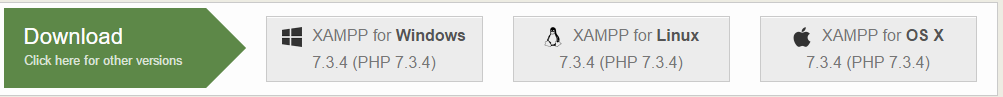
\includegraphics[scale=0.5]{figures/xampp}
\caption{Versi Terbaru XAMPP}
\end{figure}

File xampp-windows-x64-7.3.4-0-VC15-installer berukuran cukup besar, sekitar 149MB. Simpanlah file ini dimana kita inginkan.
Setelah file XAMPP sudah di download, kita akan menginstallnya dengan cara double klik pada aplikasi tersebut dan akan mucul peringatan sebagai berikut.

 \begin{figure}[h]
\centering
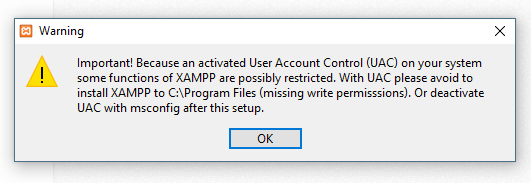
\includegraphics[scale=0.5]{figures/uac}
\caption{User Account Control}
\end{figure}

Peringatan ini berkaitan dengan keamanan pada versi Windows Vista keatas dan jika XAMPP akan di install pada folder C mungkin akan terjadi pembatasan hak akses terhadap XAMPP yang berjalan tidak normal. Silahkan klik tombol OK untuk melanjutkan install maka akan muncul jendela awal install. Silahkan klik next.

 \begin{figure}[h]
\centering
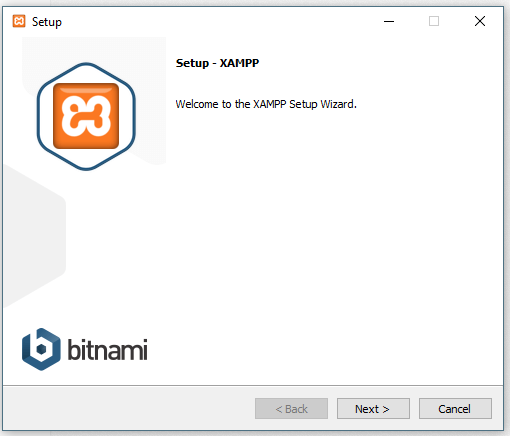
\includegraphics[scale=0.5]{figures/jendelaawal}
\caption{Jendela Awal}
\end{figure}

Jendela selanjutnya adalah Select Component. Dalam jendela ini kita dapat memilih modul atau aplikasi apa saja yang akan kita install. Dalam tahap ini kita akan menceklis semua pilihan selanjutnya klik next untuk melanjutkan.

\begin{figure}[h]
\centering
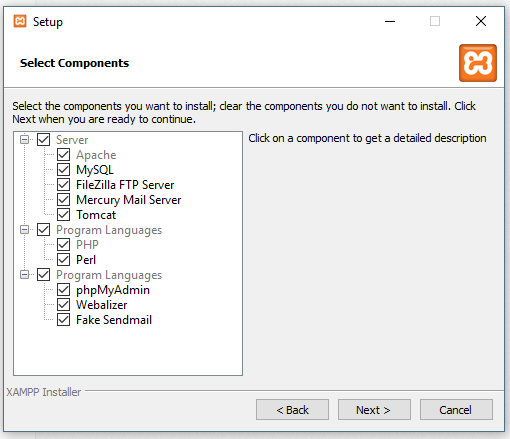
\includegraphics[scale=0.5]{figures/selectcomponent}
\caption{Select Component}
\end{figure}

Jendela selanjutnya adalah Installation Folder. Dalam jendela ini kita dapat mengubah lokasi dimana kita akan menyimpan file-file XAMPP. Sebagai contoh kita akan menyimpan file XAMPP di drive E dengan nama folder xampp agar mudah di ingat. Untuk melanjutkan klik next.

\begin{figure}[h]
\centering
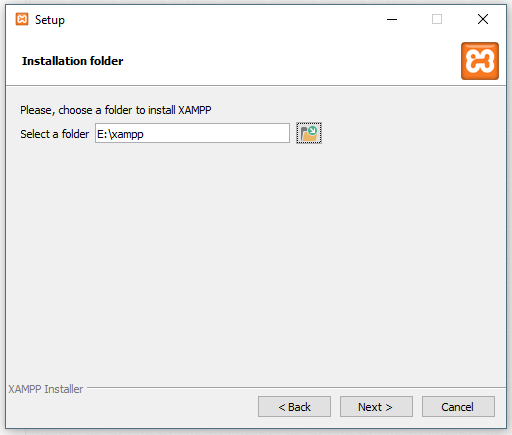
\includegraphics[scale=0.5]{figures/installationfolder}
\caption{Installation Folder}
\end{figure}

Jendela berikutnya adalah Bitnami for XAMPP. Dalam hal ini XAMPP menawarkan Bitnami sebagai cara cepat untuk install CMS seperti wordpress, drupal, dan joomla. Kemudian klik next.

\begin{figure}[h]
\centering
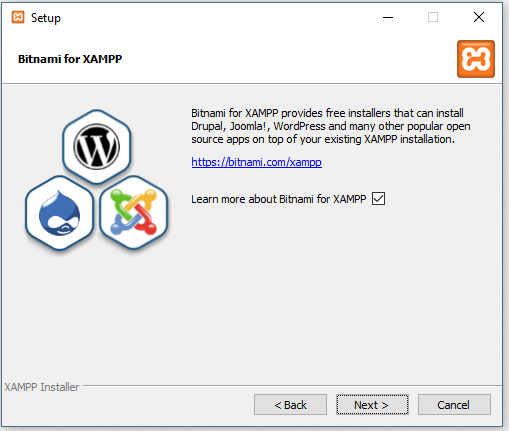
\includegraphics[scale=0.5]{figures/bitnamiforxampp}
\caption{Bitnami for XAMPP}
\end{figure}

Jendela berikutnya adalah pemberitahuan bahwa kita siap untuk menginstall XAMPP, Klik next dan XAMPP akan memulai  proses penginstallan.

\begin{figure}[h]
\centering
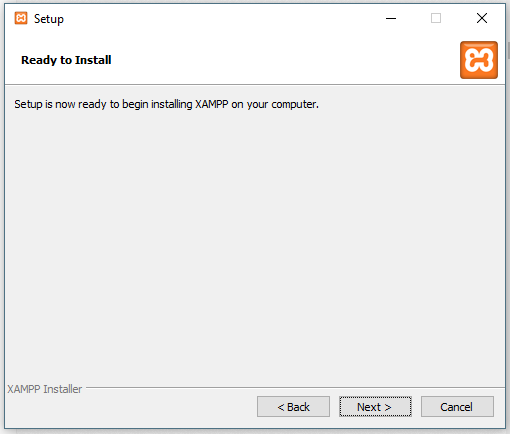
\includegraphics[scale=0.5]{figures/readytoinstall}
\caption{Ready to Install}
\end{figure}

\begin{figure}[h]
\centering
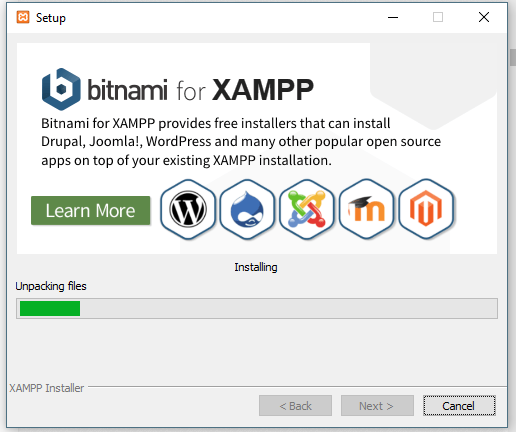
\includegraphics[scale=0.5]{figures/setup}
\caption{Proses Penginstallan}
\end{figure}

Setelah proses penginstallan hampir selesai akan muncul jendela Windows Security Alert pada gambar 5.9 karena Windows Defender Firewall mendenteksi Apache HTTP Server. Untuk lanjut klik Allow access.

\begin{figure}[h]
\centering
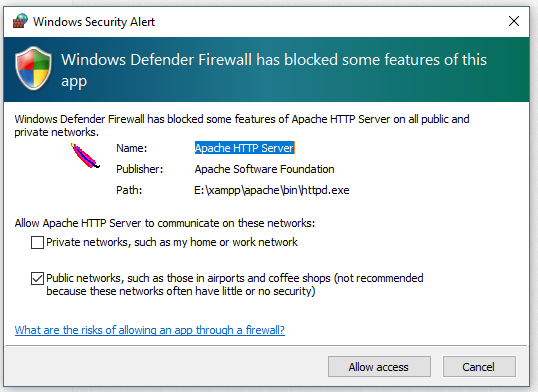
\includegraphics[scale=0.5]{figures/windowssecurityalert}
\caption{Windows Security Alert}
\end{figure}

Proses penginstallan XAMPP sudah selesai pada gambar 5.10 maka akan muncul jendela Completing, dalam bagian ini kita dapat memilih untuk langsung menggunakan XAMPP atau tidak. Jika ingin langsung memakai, ceklis pada Do you want to start the Control Panel now? lalu klik finish. Jika tidak maka hilangkan ceklis dari  Do you want to start the Control Panel now? lalu klik finish.

\begin{figure}[h]
\centering
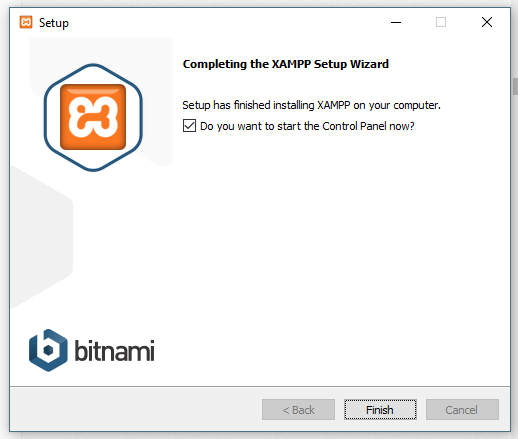
\includegraphics[scale=0.5]{figures/selesaiinstall}
\caption{Selesai Install}
\end{figure}

\subsection{Menguji Instalasi XAMPP}
Sesuai dengan namanya, jendela XAMPP Control Panel adalah jendela yang digunakan untuk mengontrol apa saja modul atau aplikasi apa saja yang ingin kita jalankan. Jika ingin membuka manual maka kita dapat membuka dengan cara dari menu Start->All Programs->XAMPP->XAMPP Control Panel. Untuk menguji instalan XAMPP ini, silahkan klik tombol Start pada modul apache dan MySQL. Jika tidak ada masalah maka akan tampil warna hijau pada bagian modul ini.

\begin{figure}[h]
\centering
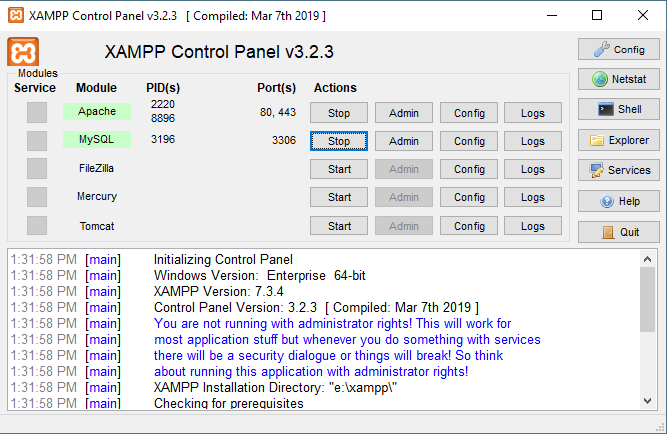
\includegraphics[scale=0.5]{figures/controlpanel}
\caption{XAMPP Control Panel}
\end{figure}

Selanjutnya buka web browser dan ketikan localhost pada address bar kemudian enter maka akan muncul dengan otomatis localhost/dashboard semuanya telah terinstall dengan baik.

\begin{figure}[h]
\centering
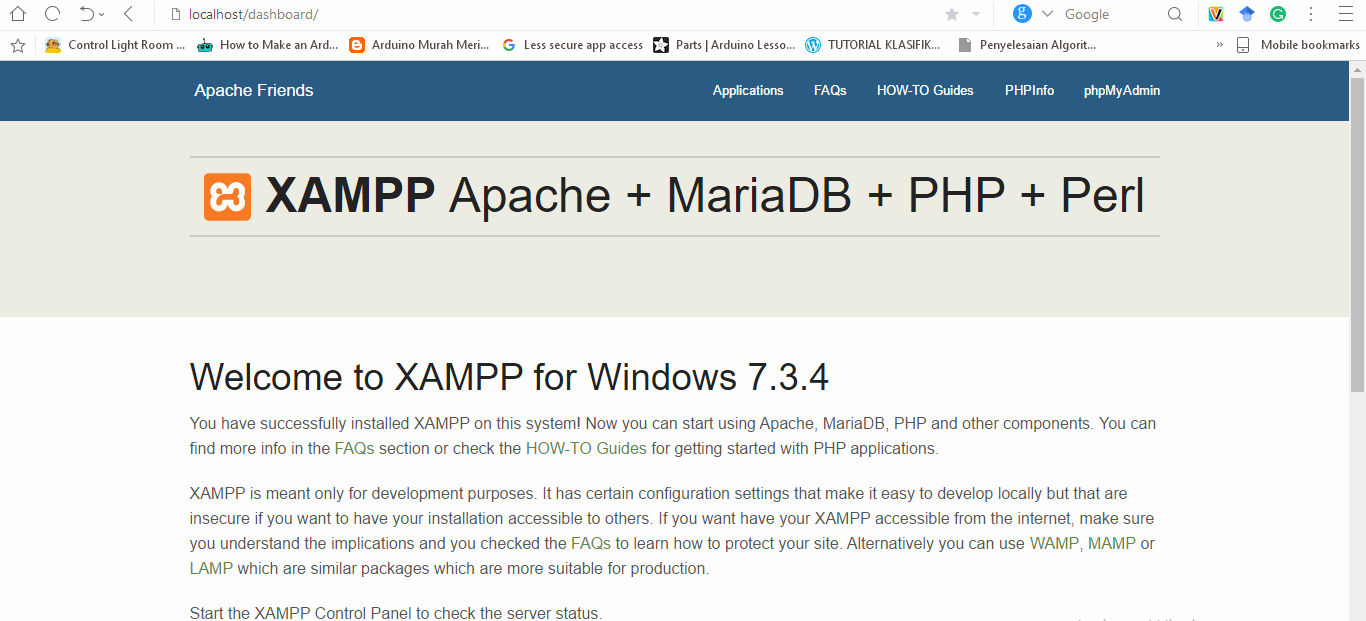
\includegraphics[scale=0.3]{figures/dashboard}
\caption{Localhost Dashboard}
\end{figure}

Jika ingin melihat versi PHP kita secara mendalam silahkan klik PHPInfo di pojok kanan atas. Disini kita dapat melihat bahwa PHP yang kita pakai sudah versi 7.3.4.

\begin{figure}[h]
\centering
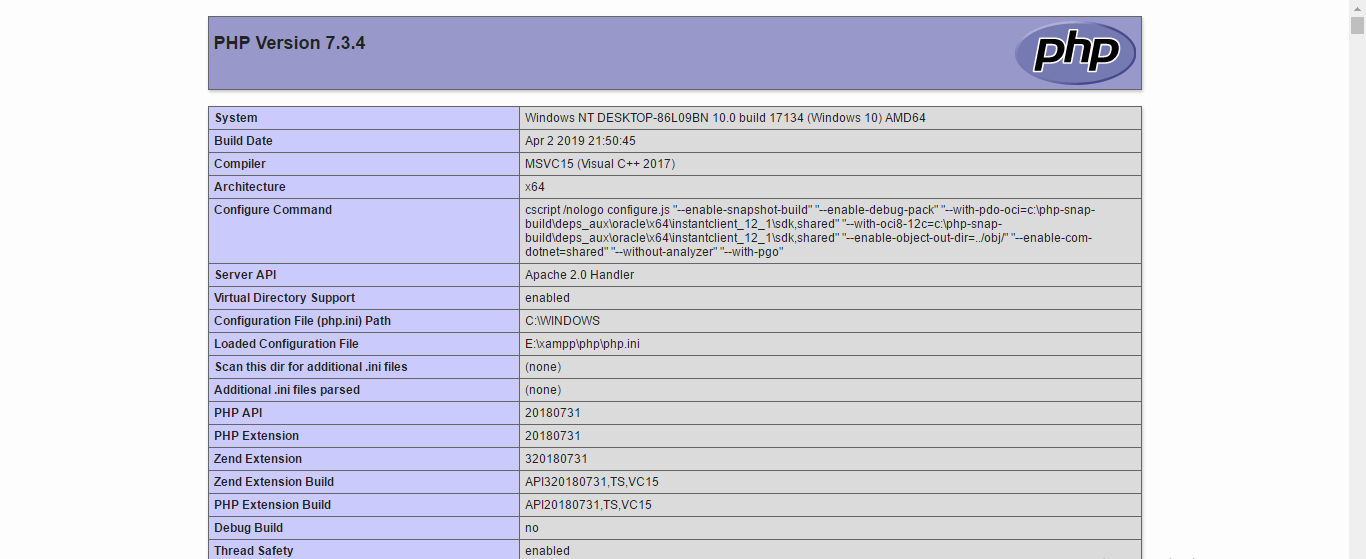
\includegraphics[scale=0.4]{figures/versiphp}
\caption{Versi PHP}
\end{figure}

\subsection{Membuat Database}
Secara umum, tipe website bisa dibedakan menjadi dua yaitu web statis dan web dinamis. Web statis adalah web yang tetap dalam arti tampilan, navigasi, dan konten tidak dapat berubah dengan otomatis. Ketika kita ingin mengupdate sebuah kegiatan akan tetapi kita harus membuka file yang aslinya. Umumnya kegiatan yang ditampillkan tetap untuk jangka waktu satu hari - satu hari. Tipe website ini biasanya hanya berupa tag html saja, jadi diperlukan database yang digunakan untuk menyimpan data.
\par
Selain memanfaatkan tag html, website yang menggunakan flash juga bisa dikategorikan sebagai web statis, meskipun ada sebagian kecil yang sudah memiliki database dalam mengelola konten tidak perlu membuka sebuah file tertentu namum hanya menambahkan pada form yang telah disiapkan dan tersimpan di database. Sama halnya dengan e-logbook ini harus ada database yang dibuat.
\begin{enumerate}
\item Untuk membuat database kita pertama kali harus membuka aplikasi XAMPP yang sudah terinstall dan klik start pada Apache serta MySQL.

 \begin{figure}[h]
\centering
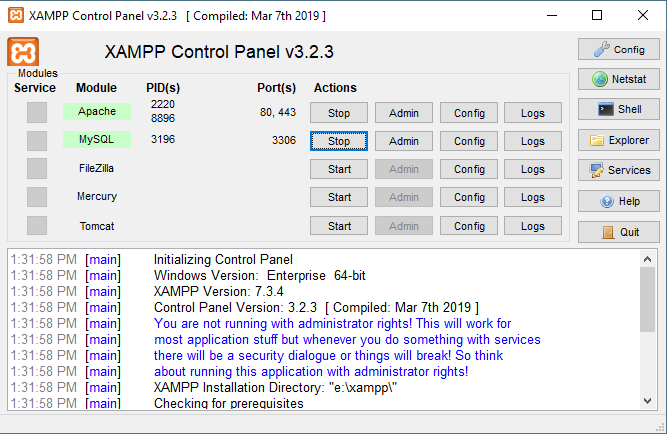
\includegraphics[scale=0.5]{figures/controlpanel}
\caption{XAMPP Control Panel}
\end{figure}

\item Jika sudah berjalan maka selanjutnya buka web browser kesayangan kita lalu ketikan https://localhost/phpmyadmin

 \begin{figure}[c]
\centering
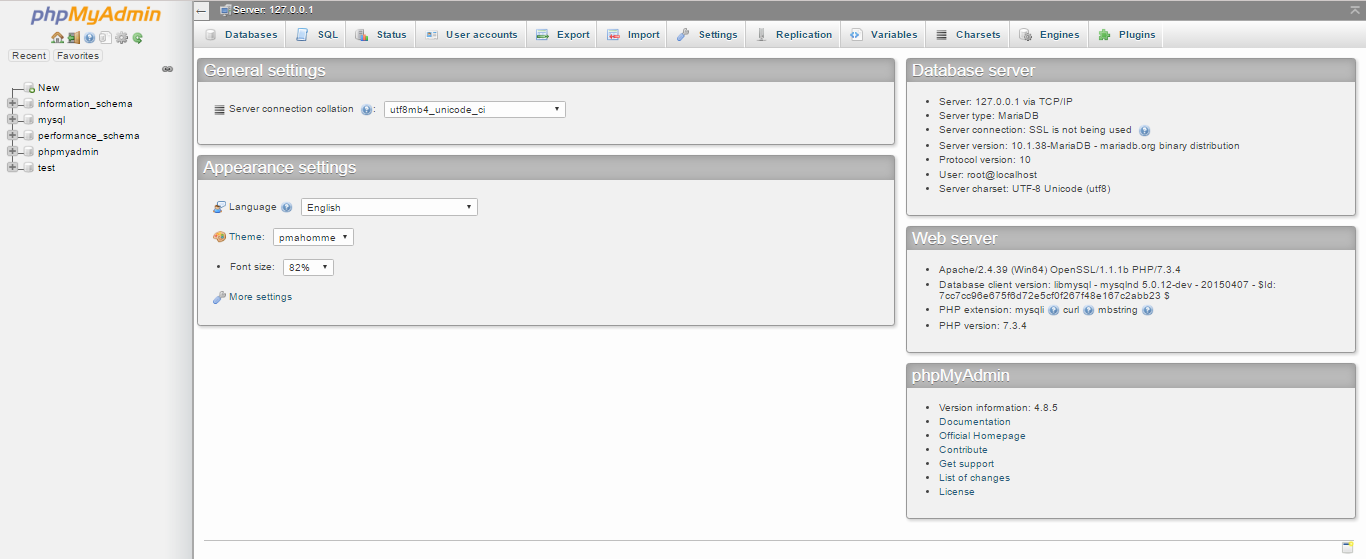
\includegraphics[scale=0.35]{figures/phpmyadmin}
\caption{Halaman Utama}
\end{figure}

\item Setelah itu, klik databases lalu ketikkan elban lalu klik create

 \begin{figure}[c]
\centering
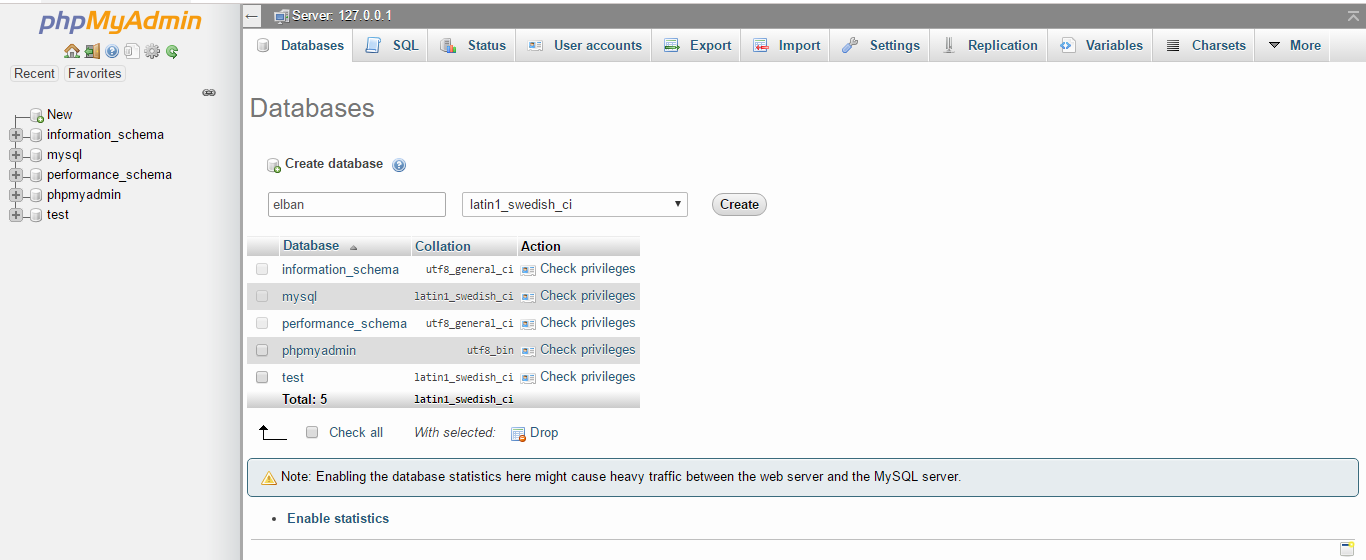
\includegraphics[scale=0.35]{figures/databases}
\caption{Create Database}
\end{figure}

\item Setelah database dibuat lalu belum ada table, klik SQL lalu masukan codingan berikut

\begin{lstlisting}
CREATE TABLE IF NOT EXISTS `logbook` (
  `id_logbook` int(10) NOT NULL,
  `tanggal` date NOT NULL,
  `petugas` varchar(100) NOT NULL,
  `vendor` varchar(100) NOT NULL,
  `penerbangan` varchar(100) NOT NULL,
  `kegiatan` varchar(500) NOT NULL,
  `point_kerusakan` varchar(200) NOT NULL,
  `target_pekerjaan` varchar(200) NOT NULL,
  `id_user` tinyint(1) NOT NULL
) ENGINE=InnoDB AUTO_INCREMENT=4 DEFAULT CHARSET=latin1;

--
-- Dumping data for table `logbook`
--

INSERT INTO `logbook` (`id_logbook`, `tanggal`, `petugas`, `vendor`, `penerbangan`, `kegiatan`, `point_kerusakan`, `target_pekerjaan`, `id_user`) VALUES
(2, '2019-03-31', 'M. Arif S, Vania & Rismayadi', 'Anto (CUPPS) Hisyam', 'Citylink KJT - KNO', 'PM di SCP 2 Inter Line 1', 'Master Clok Gate 4, XRAY BHS Internasional', 'Master Clock Gate 4', 12),
(3, '2019-03-28', 'M. Arif S & Vania', 'Anto (CUPPS) Hisyam', 'KJT - KNO (Cancelled)', 'PM', 'Master clock gate 4 off', 'Master CloCk gate 4', 12);

-- --------------------------------------------------------

--
-- Table structure for table `pegawai`
--

CREATE TABLE IF NOT EXISTS `pegawai` (
  `id_pegawai` int(10) NOT NULL,
  `pegawai` varchar(100) NOT NULL
) ENGINE=InnoDB AUTO_INCREMENT=16 DEFAULT CHARSET=latin1;

--
-- Dumping data for table `pegawai`
--

INSERT INTO `pegawai` (`id_pegawai`, `pegawai`) VALUES
(1, 'M. Arif S'),
(2, 'M. Arif S & Vania'),
(3, 'M. Arif S, Vania & Hafiz'),
(4, 'M. Arif S, Vania & Rismayadi'),
(5, 'M. Arif S & Hafiz'),
(6, 'M. Arif S & Rismayadi'),
(7, 'M. Arif S, Vania, Hafiz & Rismayadi'),
(8, 'Vania'),
(9, 'Vania & Hafiz'),
(10, 'Vania & Rismayadi'),
(11, 'Vania, Hafiz & Rismayadi'),
(12, 'Hafiz'),
(13, 'Hafiz & Rismayadi'),
(14, 'Rismayadi'),
(15, 'M. Arif S, Hafiz & Rismayadi');

-- --------------------------------------------------------

--
-- Table structure for table `user`
--

CREATE TABLE IF NOT EXISTS `user` (
  `id_user` tinyint(2) NOT NULL,
  `username` varchar(30) NOT NULL,
  `password` varchar(35) NOT NULL,
  `nama` varchar(50) NOT NULL,
  `alamat` varchar(150) NOT NULL,
  `hp` varchar(20) NOT NULL,
  `level` tinyint(1) NOT NULL
) ENGINE=InnoDB AUTO_INCREMENT=14 DEFAULT CHARSET=latin1;

--
-- Dumping data for table `user`
--

INSERT INTO `user` (`id_user`, `username`, `password`, `nama`, `alamat`, `hp`, `level`) VALUES
(1, 'admin', '21232f297a57a5a743894a0e4a801fc3', 'Luqman Nurfajri', 'Ciwarugotham', '089634530333', 1),
(13, 'vania', '081c2ce8528c443cc4be69d4096c9778', 'Vania R', 'Kertajati', '-', 1);

--
-- Indexes for dumped tables
--

--
-- Indexes for table `logbook`
--
ALTER TABLE `logbook`
  ADD PRIMARY KEY (`id_logbook`);

--
-- Indexes for table `pegawai`
--
ALTER TABLE `pegawai`
  ADD PRIMARY KEY (`id_pegawai`);

--
-- Indexes for table `user`
--
ALTER TABLE `user`
  ADD PRIMARY KEY (`id_user`);

--
-- AUTO_INCREMENT for dumped tables
--

--
-- AUTO_INCREMENT for table `logbook`
--
ALTER TABLE `logbook`
  MODIFY `id_logbook` int(10) NOT NULL AUTO_INCREMENT,AUTO_INCREMENT=4;
--
-- AUTO_INCREMENT for table `pegawai`
--
ALTER TABLE `pegawai`
  MODIFY `id_pegawai` int(10) NOT NULL AUTO_INCREMENT,AUTO_INCREMENT=16;
--
-- AUTO_INCREMENT for table `user`
--
ALTER TABLE `user`
  MODIFY `id_user` tinyint(2) NOT NULL AUTO_INCREMENT,AUTO_INCREMENT=14;
\end{lstlisting}

\end{enumerate}
